\section{Participation in the World Process}


In \emph{Saving the Appearances}, \textbf{Owen Barfield} demonstrates how the world is represented in consciousness and, moreover, how those representations alter over time. If the collective consciousness of the first men can be described as an innocence — which was destroyed through our dualist thinking — then the ultimate goal is to achieve a second innocence, or what Paul Ricoeur called a second naïveté. Barfield uses the terms ``original participation" and ``final participation". Mircea, calling it ``archaic consciousness", describes it this way:

\begin{wrapfigure}{rt}{.3\textwidth}
 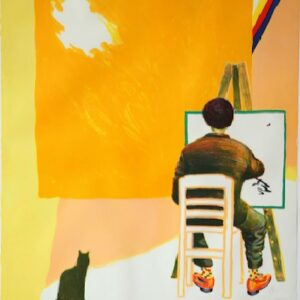
\includegraphics[scale=.5]{a20210706ParticipationintheWorldProcess-img001.jpg} 
 \end{wrapfigure}

\begin{quotex}
In \emph{imitating} the exemplary acts of a god or of a mythical hero, or simply by recounting their adventures, the man of an archaic society detaches himself from profane time and magically re-enters the Great Time, the sacred time. \flright{\emph{Myths, Dreams and Mysteries}}

\end{quotex}
Of course, the modern man, unable to take such myths at face value, does so in a different manor from the primitive man. \textbf{Paul Ricoeur} calls this re-enactment the second naïveté. In any case, knowledge of sensory space-time events can never be more than a matter of opinion (\emph{doxa}). Hence, sacred time refers to events in consciousness. \textbf{Hans Leisegang} makes this clear:

\begin{quotex}
Every myth expresses, in a form narrated for a particular case, an eternal idea, which will be intuitively recognised by him who re-experiences the content of the myth. \flright{\emph{Die Gnosis}}

\end{quotex}
\textbf{Valentin Tomberg} in \emph{Meditations on the Tarot}  points out the relationship between myths and archetypes:

\begin{quotex}
myths reveal the archetypes which manifest themselves endlessly in history and in each individual biography — they are mythological symbols pertaining to the domain of time.

\end{quotex}
\paragraph{The Starting Point}
Barfield, too, wants to breathe life into those ancient myths, which have mostly become ``dead letters" or mere verbal formulations to consent to. Barfield starts by calling attention to two misconceptions about our consciousness of the world: First an omission and then an assumption.

\begin{itemize}
\item \textbf{Omission}. The omission is neglecting to take account of the role of human consciousness in our experience of the phenomena of the world. If the physical world has no colour, smell, sound, or taste — and no physicist today would deny it — then those qualities need to come from somewhere. That is the participation of man's own mind in the creation, or evocation, of these phenomena. 
\item \textbf{Assumption}. The unexamined assumption is that human consciousness has remained unchanged throughout human history. 
\end{itemize}
Barfield is not interested in providing any metaphysic justification for these points, since his purpose is simply to describe what is. Nevertheless, a good metaphysic can provide the justification to make these views plausible.

First of all, Barfield notes that our experiences, \emph{ceteris paribus}, are essentially identical. This he calls the ``collective consciousness". Yet there is a sound explanation for that, otherwise we would be entrapped in incommunicable subjectivity. The explanation is that we all share in the World Soul, or Manas, which guarantees the identity of our sense experiences.

Then, we need to take into account that there is a larger cosmic process that organizes and unites different epochs in world history. Just as there are longer cycles, there are shorter cycles within the longer cycle. Hence, in line with Traditional cosmology, we would expect changes in the general consciousness during these cycles.

\paragraph{Four Stages}
Barfield then describes the changes in the manner of thinking over time. He begins with the ``representation" and shows how thinking changes. It is not thinking per se that changes, but rather the object of thinking. In contemporary philosophical language, Barfield is describing \textbf{intentionality.}

\begin{enumerate}
\item \textbf{Representation}: This is our sensory experience of the world. The representation IS the world; this does not mean that the world is subjective and arbitrary. 
\item \textbf{Figuration}: this is the process of converting the sensations of the world into things. 
\item \textbf{Alpha thinking}: this is the act of thinking about the things of figuration. This culminates in science which thinks about the world and organizes the things in it. 
\item \textbf{Beta thinking}: this is thinking about the previous processes and trying to understand them. This is the task typically of philosophy and metaphysics 
\end{enumerate}
Once again, there are metaphysical explanations. In order to overcome Cartesian dualism, the act of representation cannot be understood as an ``I" observing a ``world out there, right now". Rather, the representation is precisely that world; that is nondual awareness. The corollary is that there is no world unless there is someone conscious of it.

This may give you pause, but it is necessary to understand it. The famous example is: ``Does the falling tree make a sound when there is no one there to hear it?" The answer is clearly ``no". You can continue: ``Does the tree make a sight is there is no one there to hear it?" and even: ``Does the tree feel like anything if there is no one there to touch it." So whatever may be ``there", it is part of the unconscious and thus nothing like the familiar world of our senses.

Figuration basically arises from hylomorphism. Figuration answers the question: ``What is the thing that I am experiencing in my senses?" The Traditional answer is that it is the thing's essence or ``idea" in the Divine Intellect.

Alpha thinking, then, is simply the study of the things in the world, and beta thinking is the study of one's own consciousness.

\paragraph{The Recovery of Innocence}
At the figuration stage, there is a direct experience of the world, in which the person feels embedded and part of. Thought creates separation and a false ``ego" that feels separate from the world. Barfield's task, therefore, is to recapture the sense of figuration, all the while aware of how consciousness is operating.


\hfill

These are from the notes of our Summer Reading Program.



\flrightit{Posted on 2021-07-06 by Cologero }

\begin{center}* * *\end{center}

\begin{footnotesize}\begin{sffamily}



\texttt{Max Leyf on 2021-07-07 at 14:18 said: }

Thank you Cologero for the summary of Barfield's work. Some of your readers may be interested in a more extended treatment of Barfield's vision and its significance that I wrote as a part of my dissertation. The article should be accessible here:

\url{https://www.cosmosandhistory.org/index.php/journal/issue/view/39}

The entire dissertation, which integrates Barfield's thought with the theory and method of knowledge developed by Goethe and Rudolf Steiner, is also available:

\url{https://theoriapress.wordpress.com/2020/12/02/new-publication-the-redemption-of-thinking/}

Anyone with special interest in this subject is welcome to contact me.

My thanks again to you for all of your offerings.

Max Leyf


\end{sffamily}\end{footnotesize}
